\documentclass[11.5pt, oneside]{article}   	% use "amsart" instead of "article" for AMSLaTeX format
\usepackage{geometry}                		% See geometry.pdf to learn the layout options. There are lots.
\geometry{letterpaper}                   		% ... or a4paper or a5paper or ... 
\geometry{legalpaper, portrait, margin=1in}
\usepackage[parfill]{parskip}    			% Activate to begin paragraphs with an empty line rather than an indent
\usepackage{graphicx}				% Use pdf, png, jpg, or eps§ with pdflatex; use eps in DVI mode
\usepackage{amssymb}
\usepackage{multicol}
\usepackage{abstract} 
\usepackage{graphicx}
\usepackage{caption}

\title{Saito: A Big-Data Blockchain with Proof-of-Transactions}
\author{David Lancashire}
\date{February 11, 2019\\v. 3.0.1}
\begin{document}
\maketitle


\begin{onecolabstract}
Saito is a blockchain designed to process terabytes of data every day, a level of scalability achieved by coupling a transient ledger to a proof-of-transactions mechanism that pays the network for collecting transaction fees. Saito continually evolves towards an optimal network structure while eliminating sibyl-attacks, fee-recycling attacks, block-withholding attacks and more. It provides a decentralized and efficient platform on which to build bandwidth-intensive Internet applications like email, social networks, decentralized chat, cryptocurrency payment channels, and much more.
\end{onecolabstract}


\begin{multicols}{2}
Saito is a cryptocurrency designed for applications that need to broadcast large amounts of data across a blockchain. It can be used to build decentralized versions of most Google services, along with un-astroturfable Internet forums, social networks, pay-to-play websites, distributed key registries that are secure from MITM attacks, payment channels, and more.

We believe the practical limit for a Saito blockchain today is on the order of 100 TB of data per day, and advances in routing capacity will push this to the petabyte level within a few years. In order to understand how this is possible, it is necessary to discuss the nature of the scaling problem. This is covered in the next section before we move on to explain the solution.

1. THE PROBLEM

The problem with blockchain scaling is not at the network technology layer. At time of writing, data centres around the world are implementing 400 Gbps network switches while 100 Gbps connections are becoming standard even in lower-tier colocation facilities. If we had the resources to pay for the necessary equipment there is nothing technically stopping us from building a blockchain that is as decentralized as the public Internet backbone.

Ensuring that people can pay for the network requires solving two problems on the incentive layer. The first is that the cost of operating the blockchain needs to be kept in check so that it is always profitable to run. The second is that the network needs to ensure that the network actually incentivizes people to pay for network equipment.

The first problem exists because all non-Saito networks get more expensive to operate the more data they process. No matter how much data developers push to second-layer networks, and how frugal their applications are at publishing data on-chain, adding data to a blockchain increases the costs of supporting the network to every participant on the network. 

There is a point at which the cost of storing the blockchain will exceed the value of operating it. The more data.

Discussing this problem in the original bitcoin implementation, Satoshi Nakamoto stated that "the only solution is not to care."  This approach -- ignoring the problem -- is not a solution. Sadly, the fact that it is typically ignored by developers has lead the entire community to believe that it is not actually an important problem to solve. 

Advocates of on-chain scaling believe that growth will be limited. While this may be right for smaller networks like bitcoin, this is an unsolved problem that needs to be fixed in order to run high-throughput blockchains like Saito.


The Saito network achieves scalability by paying for it. As unlike other blockchains, in Saito revenue is given directly to the nodes running the peer-to-peer network instead of a separate class of "miners" or "stakers" who are expected but not incentivized to pay for what the network needs. This solves the fundamental economic problem frustrating scaling. In addition, Saito introduces a sophisticated data-pruning technique that lets market forces price the cost of on-chain data storage.





No blockchain has a solution to problem.

BTC developers suggest that the solution is to cap the blocksize and push transaction and data traffic to secondary network layers such as the Lightning Network. This is not an acceptable solution for many reasons. Not only can upper-layer networks not provide the universal-broadcast features that data applications need, but limiting blocksize limits fee volume. Every  that the total amount of network security is driven by fee volume. The most secure network will be the one that is capable of processing. It is far preferable to solve teh scaling problem and have a high-security network than .







What limits network growth is the fact that no existing consensus mechanism pays directly for network load. In the past, developers have waved away this limitation, claiming that as long as {\textit{someone}} is earning money from the network they will pay all costs needed to support it. Yet this is not the case, for all proof-of-work and proof-of-stake blockchains have two collective action problems that lead to known market failures: a tragedy-of-the-commons problem that lead to blockchain collapse, and a free-rider problem that incentivizes an under-provision of network infrastructure. Both problems grow increasingly incapacitating as bandwidth and storage costs rise.

The tragedy-of-the-commons problem occurs when nodes may accept payment today in exchange for promises of work done by others tomorrow. In addition to starving networks of revenue to carry out the promised work, this problem leads to transaction mis-pricing, as users do not need to pay fees reflecting the true cost of network processing. The fundamental nature of this problem is self-evident from the way Satoshi's solution is "not to care," an unacceptable attitude for a high-throughput network.

Eliminating the tragedy-of-the-commons problem requires that all nodes which collect fees in exchange for processing transactions must fully bear the cost of processing those transactions for as long as they remain on the blockchain. In practice this means we need an elegant pruning mechanism that lets market forces rather than developers determine the cost of "rent". Additionally, our mechanism must defer fee collection so that payments are meted-out over time to whichever nodes continue to run the network. Our solution accomplishing this is described fully in Section 2.

The free-rider problem is more subtle. Because proof-of-work and proof-of-stake mechanisms reward mining and staking activities exclusively, these two classes of networks strictly punish nodes which spend funds supporting public network operations (sharing blocks, creating merkle-root proofs for lite-clients, propagating transactions rather than hoarding them).  Although it is often claimed that participants in a public network will need to do this (as otherwise the network cannot earn money), economic incentives in fact strictly punish altruism. If any major bitcoin miner is so foolish as to spend 80 percent of its revenue to support a terabyte-level public network, any miner that can get away with paying less will eat its counterparty's market share by pouring its additional profits into extra hashpower.

In economics, the only solution to the free rider problem is eliminating open access to the network in question, ensuring that only those who pay to support a public good receive the benefits from it. This is the underlying reason existing scaling proposals for POW and POS networks necessarily involve either privatizing layers of the public network (cf. BloxRoute, FALCON, FIBRE) or closing off open access to payment mechanisms through the creation of governance structures which "segment and subsidize" the network, defining classes of nodes which are eligible to collect a payments through the introduction of governance layers.

Neither approach offers an acceptable trade-off for a public blockchain, as the open access properties of the network are necessary for its decentralization and censorship-resistance. Building a blockchain that can process the massive amounts of data required by Internet-scale applications thus requires a better consensus mechanism, one that ends the practice of rewarding ancillary "work" like mining and staking and instead builds its security function around the actual work that delivers value in the network. 

2. THE TRANSIENT BLOCKCHAIN

The "transient blockchain" is a form of data-pruning that solves the tragedy of the commons problem completely. The principle behind it is simple: nodes in the network may delete the oldest blocks in their ledger at predictable intervals ("genesis periods"). At the extreme of a blockchain designed to handling global email traffic, the genesis period may be as short as 24 hours.

This method of chain management is essentially a form of pruning where the UTXO slips become unspendable after a certain number of blocks, with this restriction enforced by the consensus rules of the blockchain. With old transactions removed at roughly the same rate that new transactions are added, it becomes possible for participants in the blockchain to price the true cost of transaction inclusion to maintain the network in a steady state.

This solution can be further improved by adding "automatic transaction rebroadcasting" to the consensus layer. Under these additional restrictions, nodes which create new blocks must "re-broadcast" transactions which have fallen off the chain which meet whatever criteria the network sets as the requirement for re-inclusion.

It is trivial to see that a transient blockchain that auto-rebroadcasts all of its data is identical to a permanent ledger: rebroadcasting in such a system is simply a form of bookkeeping. So why do it? The importance of the mechanism is that it creates a vector for the consensus layer to introduce market forces. This is done by charging rebroadcast transactions a multiple of the average transaction fee paid by the average fee paid by new transactions, ideally measured with a smoothing curve to prevents fluctuations from disrupting the network.

Old and new transactions now compete for inclusion through market mechanisms. As the cost of adding new transactions to the network rises, so does the cost of maintaining old data on-chain. The least valuable data is driven off the network first when the network hits its capacity limit, and it simultanously becomes impossible for nodes to "take the money and run" -- earning recurring fees from older transactions requires the work demanded of active block producers. Transactions can be priced accurately on-chain even as storage times approach infinity.

Under this system, the burden of archiving the network history passes -- as it does in the consumer Internet -- from the routing nodes in the network to the servers and users that actually care about the data. The blockchain becomes a flexible broadcast tool instead of an expensive database, and the cost of using the network is lower for everyone as transactions which simply need one-time data propagation (i.e. most data-sharing applications) do not need to pay inflated prices for permanent storage.

While the tragedy-of-the-commons dilemma is thus resolved, this method does not solve the free-rider issued created by using mining or staking as measures of "work". To solve those problems a new consensus mechanism is needed, one we call proof-of-transactions.

3. PROOF-OF-TRANSACTIONS

Under proof-of-transactions any node can create a block at any time provided it includes enough fee-paying transactions to cover the cost of a "burn fee" set by the consensus rules of the blockchain. This "burn fee" is set to a high value immediately after a block is published and decreases gradually over time until it hits zero, at which point even a block containing no fee-paying transactions will be considered valid.

Importantly, in order to prevent all nodes from simultaneously producing blocks, the measure of "work" Saito uses is not the absolutely value of the transaction fee but rather the "usable value" of the fee, a number which drops with each hop the transaction makes across the network. Cryptographic signatures affixed to transactions allow all nodes to verify the "usable value" of each transaction in the block. And nodes are prohibited from using any transaction not routed expressly to them to pay the network burn fee.

In this design, the burn fee is a measure of the "work" involved in efficiently sourcing fee-paying transactions. This choice gives proof-of-transactions the same security properties as proof-of-work systems. Because the resources available to produce blocks increase as the total volume of transactions grows, and because nodes will generally issue blocks as soon as it becomes profitable for them to do so, the pace of block production in Saito is determined by the overall volume of transaction fees in the network, as shown below:

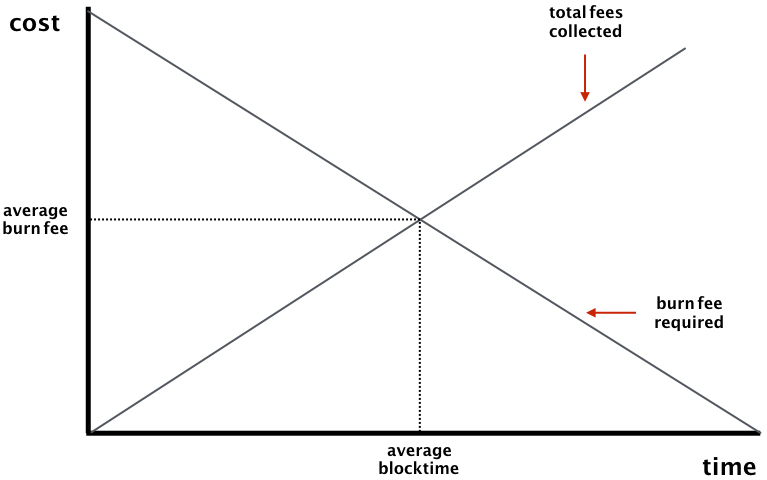
\includegraphics[width=.45\textwidth]{saito2.jpeg}

In practice, the only way for an attacker to rewrite a Saito-class chain is to spend their own money to create a competing a chain -- honest nodes thus route transactions and produce blocks for free while attackers must spend real money on what can only be temporary attacks. Security is also defended by one hundred percent of transaction fees rather than merely fifty-one percent. Figure 2 illustrates that producing blocks at a faster pace than the main chain requires outspending the rest of the network as a whole.

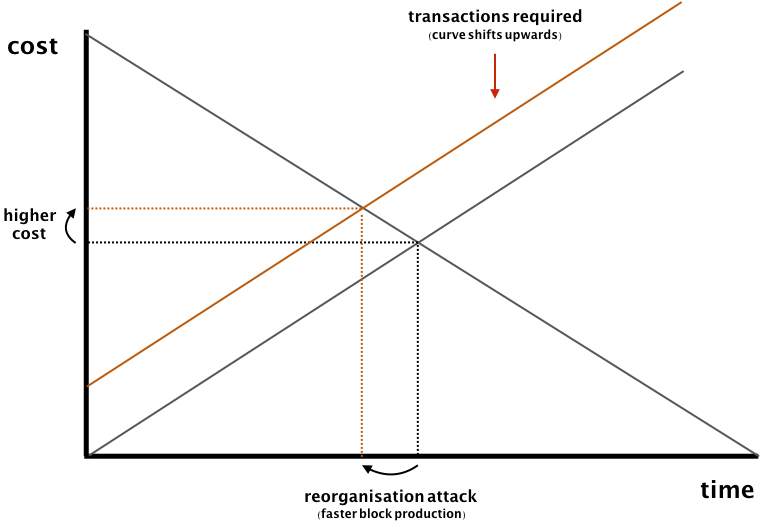
\includegraphics[width=.45\textwidth]{saito3.jpeg}

For reasons that are outlined later in this description, Saito forces attackers to pay the entire burn fee rather than just cover the marginal difference over the amount included in the main chain. The network also increases the cost of attacks over time by adjusting the burn fee upwards to keep blocktime constant as transaction volume grows. This delivers comparable security to Bitcoin in the sense that the cost of a chain-reorganization attack can always be quantified, and users that require significant guarantees of non-reversibility can calculate the expense of re-writing the chain and wait the appropriate number of confirmations

The major problem with this lies in the consequences of requiring nodes to burn fees to produce blocks. Not only does the network lack a mechanism to pay for its own operation, but the deflationary forces it unleashes will eventually destroy the on-chain economy:

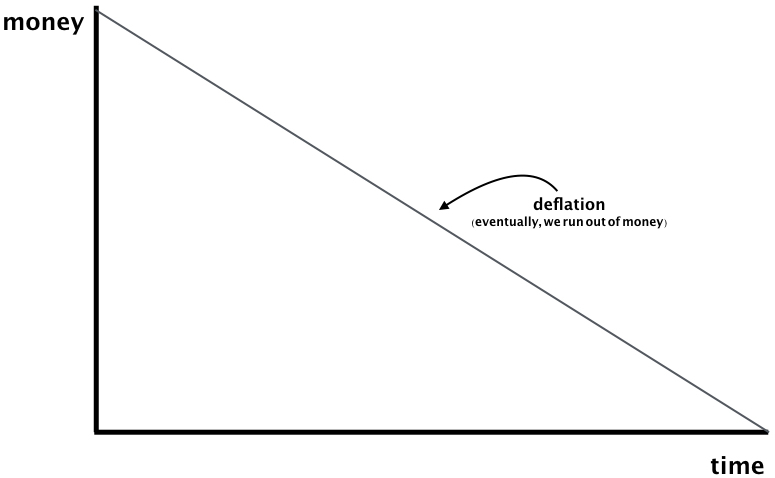
\includegraphics[width=.45\textwidth]{saito4.jpeg}

Avoiding a deflationary crash requires a secure method for token injection. But how can we do this? Saito cannot follow in the footsteps of POW and POS and simply hand the network fees directly to the block producer: doing so would eliminate the entire point of having a burn fee and enable fee-recycling attacks on the network. Splitting the fees between various nodes is a better option as it guarantees a deadweight loss on attackers without disincentivizing honest nodes, but how can we select winners in a secure fashion? 

The ideal solution is picking one or more routing nodes based on a random number that cannot be influenced by any of the participants in the network. But how can we source this randomness? The network cannot use any variable associated with the block itself since as long as the block-producing node has any influence over the random number generation a savvy attacker can sibyl the network for profit and/or simply game the token-issuing mechanism, reducing our security mechanism into a thinly-disguised proof-of-work with free-rider attacks on the payment mechanism.

The solution to this problem, outlined in the section below, involves the re-injection of the burn fee back into the network through a process that cannot be coopted by any of the players in the network. We achieve this through a zero-sum competition between bandwidth-expending nodes and CPU-expending miners in the network in a battle over the "paysplit" of the network.

4. PAYSPLIT

Whenever a node produces a block, it collects any profit it can and bundles all remaining fees into a "golden ticket" that contains (1) a computational puzzle for miners to solve, and (2) a vote to increase, decrease, or hold constant the "paysplit" of the network (the percentage of all golden tickets that are paid out to miners). By default, these tickets are included in all blocks produced. Miners listening on the network then choose which blocks to solve and -- should they find a solution to the cryptographic puzzle -- propagate their solution back into the network as a regular fee-paying transaction. In addition to a proof-of-solution, these miner transactions also include a separate vote on whether to increase, decrease, or hold constant the difficulty of the computational puzzle.

The golden ticket system can be visualized as follows:

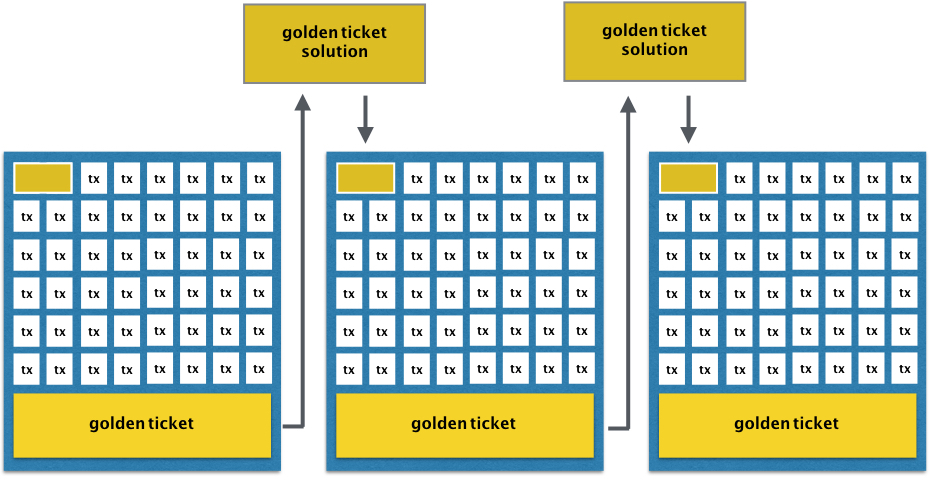
\includegraphics[width=.45\textwidth]{saito7.jpeg}

In order to increase the security of the blockchain, we specify that only one solution may be provided for any golden ticket, and that any solution must be included in the very next block to be valid. If these conditions are met, our two votes take effect and the funds that were burned the previous block are now released back into the network, split between the miner that found the solution and a random node in the peer-to-peer network. In the event a "golden ticket" is not solved, the burned funds will eventually fall off our transient blockchain, at which point they can be recycled back into our economy in the coinbase of another golden ticket.

This game is counterintuitive to many blockchainers because it separates the act of "producing blocks" from the act of "issuing tokens". This is also why it succeeds where other approaches fail: the key challenge in securing a blockchain is not to making it difficult to produce blocks (an impossible challenge) so much as to ensure that it is always prohibitively expensive.

The purpose of the voting mechanism is to put all actors into a delicate dance requiring collusion and cooperation alike. While both nodes and miners want at least one solution per golden ticket (because otherwise no-one gets paid), their interests otherwise diverge: miners prefer a high paysplit and high difficulty level, while nodes prefer a low paysplit and low difficulty level. Given that votes must pass between both players to change consensus settings, Saito creates a Mexican standoff where both groups must constantly trade-off their individual short-term against their collective long-term interests.

As an aside, we should note that a version of Saito is possible in which network paysplit is hardcoded. In this "Saito-Lite" version of our mechanism, the golden ticket system still imposes a deadweight loss on attackers (routing nodes lose the miner portion of the fee, miners lose the routing portion of the fee). As paysplit flexibility is beneficial for warding off attacks in some situations (increasing network difficulty in real-time can drive up the cost of attacks and speed up block production), we believe the hardcoded version is only preferable if evidence shows that the highly-paid nodes in our high-throughput network cannot exhibit the bounded rationality necessary to maintain the security of their own revenue streams.

Regardless of whether the network operates with a flexible or hardcoded paysplit, it can be seen that the paysplit mechanism determines the security of the system. While honest nodes earn income in exchange for fee-collection and do not mind if a portion of those fees are allocated to security providers, attackers must pay the entire cost of a block and then bear the deadweight losses that the golden ticket mechanism imposes on their ability to "recapture" spent funds and "recycle" them in circular attacks on the blockchain. The security of the system rises with the guaranteed loss that the system will impose on attackers.

There are many variants of the Saito system, such as the replacement of our mining puzzle with a proof-of-stake or algorand-powered node-selection algorithm. Regardless of how the lottery holders are selected, the key insight is that routing nodes that have miner support will produce blocks at a faster rate and be more profitable than those which do not. Miners who have the support of full-nodes will also be more profitable as well. This introduces self-balancing market forces: excessive profits in any sector of the network will attract competition that will drive down profits through the self-interested behavior of the new participants who are entering the network.

In a classic Saito deployment, the optimal strategies of collusion and defection are determined by the market structure surrounding the economics of bandwidth and mining provision. The economic design encourages convergence towards an equilibrium point at which the security provided is optimal for both nodes and miners. A useful thought experiment for those new to the mechanism is exploring how the security of this two-player system degrades to offer only bitcoin-level security as the paysplit approaches the extreme values of zero and one.

The system can also be further improved. Since we acknowledge that any level of security negotiated between routers and miners is arbitrary and may not reflect the needs of the applications on the network, Saito takes the final step of allowing users to tag all of their transactions with an optimal paysplit vote. Should a user-originated transaction contain such a vote, consensus rules dictate that it can only be included in a block which votes in the same direction. Users who choose to take sides in the ongoing struggle between nodes and miners thus sacrifice the reliability and speed of transaction confirmation in exchange for marginal influence over how the network allocates resources for block production, and thus the long-term trade-off that that the network makes between allocating funding for bandwidth and security providers.


5. ADDITIONAL SECURITY

Saito takes additional steps to secure the network. In order to deter sybilling, the nodes in our network sign transactions as they propagate through the network, adding to each an unforgeable history of the path it takes from its point of origin to its point of confirmation. Each hop a transaction takes decreases the percentage of the transaction fee that nodes can allocate to paying their burn fee. We also specify that nodes cannot pay burn fees using transactions that do not include them in their transaction path. This allows the network to defend itself from attack by refusing to send transactions to malicious participants.

In order to ensure that nodes cannot influence the distribution of funds from the golden ticket, we also specify that the node in the peer-to-peer network which wins the routing share of the golden ticket is selected using a random variable sourced from the miner solution, with the winner selected from the pool of nodes contained in the transaction propagation paths found in the previous block, and with each participant's chance of winning adjusted to reflect the proportional weight of the "usable fees" each routed into said block.

These restrictions enforce that all nodes are paid in proportion to the "value" they have contributed to the network, eliminating hoarding as viable strategy and making participants indifferent as to whether they themselves produce a block or whether they simply route a transaction to a block producer deeper in the network.

These restrictions also secure our network from common attacks in other cryptosystems which -- oddly -- are not commonly recognized as attacks. In Saito, for instance, transactions are naturally valuable to nodes which participate in the P2P network and useless to attackers who lurk on the edges. Fee-sourcing and transaction harvesting attacks are also impossible: the fact that nodes must participate in the P2P network to harvest transactions defends us against subtle attacks like those posed by the bitcoin FIBRE network, a closed-access network which benefits its participants by undermining the profitability of nodes in the peer-to-peer network. Sybilling becomes an unprofitable strategy because it necessarily adds hops in transaction routes, making attackers visible to the network and providing an evolutionary mechanism whereby weaker nodes that permit themselves to be sybilled will necessarily operate at a loss. Only nodes which monitor their economic relationships with their peers and strive to improve the value they bring to the network will survive long-term.

Security is also reinforced by the competitive economic structure of our game in fascinating ways. Note that if network security falls too low, participants are incentivized to increase it by voting to pay miners more. Not only do the rules for rewriting the longest-chain require alternate chains to have equal or greater mining difficulty, but increasing paysplit increases the volume of fees needed to attack the network by inducing competition in the golden ticket system fosters fee-competition among miners who now must pay a premium to have their solutions included over those of their peers. Even in situations where the network is not under active attack, the miner/node battle over the paysplit vote also serves a defensive "canary in the coalmine" function, encouraging miners to issue their own pro-miner blocks if they control enough hashpower to support the block.

Finally, we note that as unlike POS and POW networks where stealth attacks are possible and can be easily hidden across multiple network pools, the public nature of the paysplit and difficulty variables makes attacks on the Saito network fully transparent. And of course network nodes can respond to attacks in real-time by routing transactions away from attackers and towards honest defenders, weaponizing the routing network to further disincentivize attacks and strengthen network defenses.

6. SUMMARY

Saito is a solution for building a massively-scalable blockchain. We achieve this scalability not through algorithmic tweaks to existing technologies, but rather by solving the deeper and more profound economic problem that affects all existing blockchain designs, by making it expensive rather than merely difficult to produce blocks.

Those who pour over the technical details of the Saito network will find embedded in it at least seven major innovations in blockchain technology: the transient blockchain, the burn fee, the usable transaction fee, the golden ticket system, our secure multi-party voting mechanism, automatic transaction rebroadcasting, and the chain of cryptographic signatures we embed in transactions to identify and reward productive nodes in the network. We have secured patent protection on these techniques and look forward to working with others on rolling out an open public network that can use these techniques to achieve mass-data on-chain scalability.

Seeking more information? We encourage everyone to visit our website (http://saito.tech), where we maintain a working demo of the network, a roadmap outlining our development plans, links to downloadable software, and tutorials that can help anyone get started building Saito applications *today*.         

\end{multicols} 
\end{document}
